\section{Конструкторская часть}

\subsection{IDEF0}
Концептуальная модель программы представлена в нотации IDEF0 на рисунке \ref{pic:idef0-1}

\myImage
{schemes/idef0.pdf}
{Концептуальная модуль системы в нотации IDEF0.}
{pic:idef0-1}


\subsection{Грамматика языка tinyc}
Грамматика языка tinyc \ref{lst:grammar} является крайне упрощённым вариантом грамматики языка Си.

\lstinputlisting[caption = Грамматика языка tinyc]{code/tinyc.g4}\label{lst:grammar}

Так как эта грамматика не удовлетворяла требованиям курсовой работы, она была дополнена элементами грамматики Си. Были добавлены следующие элементы синтаксиса:
\begin{itemize}
    \item недостающие арифметические операции с учётом приоритетов действий;
    \item объявления и инициализация переменных;
    \item поддержка многомерных статических массивов;
    \item комментарии.
\end{itemize}
Полная дополненная грамматика приведена в Приложении А.

\subsection{Обход синтаксического дерева}
Исходная программа преобразовывается в синтаксическое дерево при помощи кода, сгенерированного ANTLR4 для описанной грамматики. Обход всех узлов данного представления позволяет сгенерировать LLVM IR.

Рассмотрим синтаксическое дерево на примере изображения \ref{div7:tree}.
\begin{figure}[h!]
	\begin{center}
		{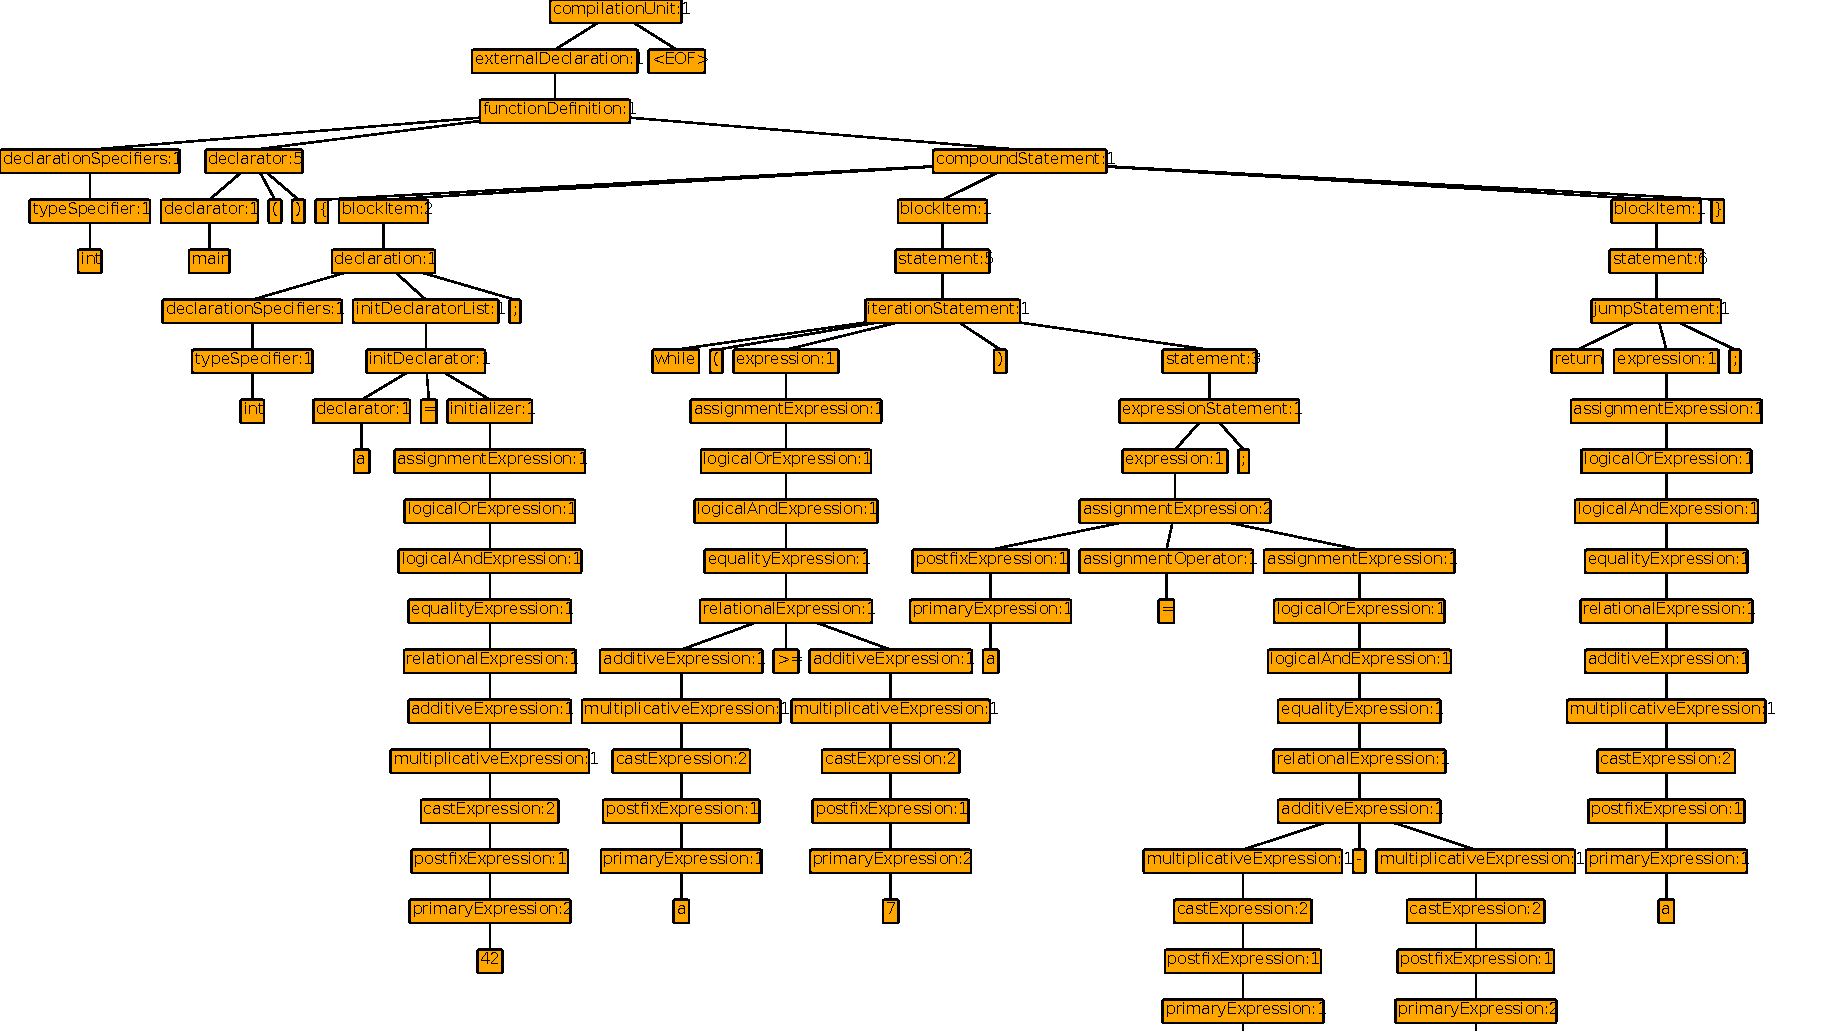
\includegraphics[width=0.85\textheight, angle = 90]{img/div7.pdf}}
		\caption{Пример визуализации синтаксического дерева.}
		\label{div7:tree}
	\end{center}
\end{figure}
\pagebreak

Данная визуализация получена использованием утилиты \textbf{antlr4-parse} для следующей программы, вычисляющей остаток от деления числа на 7.

\lstinputlisting[caption = Пример программы (остаток от деления на 7)]{code/div7.c}\label{lst:fib}

\subsection{Генерация LLVM IR}
Сгенерировать промежуточное представление LLVM можно путём обхода всех узлов синтаксического дерева. Каждый узел может создавать новые инструкции, блоки, функции и т.п. в зависимости от его типа и дочерних узлов. Рассмотрим пример обработки узла \textbf{iterationStatement}, грамматика которого показана в выражении \ref{iterationStatement}. На рисунке \ref{pic:while} приведена схема алгоритма генерации кода для цикла while.

\begin{equation}
    \label{iterationStatement}
    \text{iterationStatement: While '(' expression ')' statement;}
\end{equation}

\myImage
{schemes/while.pdf}
{Схема алгоритма обработки узла iterationStatement.}
{pic:while}

\subsection*{Вывод}
В данном разделе была предоставлена концептуальная модель метода компиляции в нотации диаграммы IDEF0. Приведена грамматика tinyc, описаны предпринятые расширения. Описаны работы frontend часть разрабатываемого компилятора.

\pagebreak
